% SIAM Article Template
\documentclass{siamart0516}
\usepackage{subfig}
\usepackage{forest}
\usepackage[section]{placeins}
\usepackage[export]{adjustbox}
\usepackage[title]{appendix}

\newcommand{\lp}{\left(}
\newcommand{\rp}{\right)}

\newcommand{\R}{\mathbb{R}}
\newcommand{\N}{\mathbb{N}}
\newcommand{\Z}{\mathbb{Z}}
\newcommand{\Q}{\mathbb{Q}}
\newcommand{\C}{\mathbb{C}}
\newcommand\supp{\mathop{\rm supp}}

%%


\newcommand{\prop}[2]{\textsf{#1}(#2)}

\newcommand{\vect}[1]{\mathbf{#1}}
\newcommand{\plotwidth}{0.45}
\newcommand{\WRP}{\par\qquad\(\hookrightarrow\)\enspace}
\newcommand{\ARP}{\par\qquad\ \enspace}
\DeclareMathOperator*{\argmax}{argmax}

%%%%% custom commands for this paper
\newcommand{\nmax}{N}
\newcommand{\bigo}{\mathcal{O}}
\newcommand{\child}[1]{\textsf{child}$_{#1}$}
\newcommand{\weight}[1]{w\textsubscript{#1}}
%%%%%


% Information that is shared between the article and the supplement
% (title and author information, macros, packages, etc.) goes into
% ex_shared.tex. If there is no supplement, this file can be included
% directly.
% SIAM Shared Information Template
% This is information that is shared between the main document and any
% supplement. If no supplement is required, then this information can
% be included directly in the main document.


% Packages and macros go here
\usepackage{lipsum}
\usepackage{amsfonts}
\usepackage{graphicx}
\usepackage{epstopdf}
\usepackage{algorithmic}
\ifpdf
  \DeclareGraphicsExtensions{.eps,.pdf,.png,.jpg}
\else
  \DeclareGraphicsExtensions{.eps}
\fi

% Add a serial/Oxford comma by default.
\newcommand{\creflastconjunction}{, and~}

% Used for creating new theorem and remark environments
\newsiamremark{remark}{Remark}
\newsiamremark{hypothesis}{Hypothesis}
\crefname{hypothesis}{Hypothesis}{Hypotheses}
\newsiamthm{claim}{Claim}


%\newcommand{\TheTitle}{An adaptive partition of unity method for Chebyshev polynomial interpolation on Hypercubes} 
%\newcommand{\TheAuthors}{Kevin W. Aiton, Tobin A. Driscoll}


% Sets running headers as well as PDF title and authors
\headers{Adaptive partition of unity}{Kevin W. Aiton, Tobin A. Driscoll}

% Title. If the supplement option is on, then "Supplementary Material"
% is automatically inserted before the title.
\title{Preconditioned nonlinear iterations for overlapping Chebyshev discretizations with partition of unity \thanks{Submitted to the editors May 1, xxxx.
\funding{This research was supported by National Science Foundation grant DMS-1412085.}}}

% Authors: full names plus addresses.
\author{Kevin W. Aiton, Tobin A. Driscoll}

\usepackage{amsopn}
\DeclareMathOperator{\diag}{diag}


%%% Local Variables: 
%%% mode:latex
%%% TeX-master: "ex_article"
%%% End: 


% Optional PDF information
\ifpdf
\hypersetup{
  pdftitle={\TheTitle},
  pdfauthor={\TheAuthors}
}
\fi

% The next statement enables references to information in the
% supplement. See the xr-hyperref package for details.

\externaldocument{ex_supplement}

% FundRef data to be entered by SIAM
%<funding-group>
%<award-group>
%<funding-source>
%<named-content content-type="funder-name"> 
%</named-content> 
%<named-content content-type="funder-identifier"> 
%</named-content>
%</funding-source>
%<award-id> </award-id>
%</award-group>
%</funding-group>

\begin{document}

\maketitle

% REQUIRED
\begin{abstract}
We are doing adaptive multivariate approximations, and it works pretty well. This is a working abstract.

\end{abstract}

% REQUIRED
\begin{keywords}
  partition of unity, Chebyshev interpolation, Chebfun, overlapping domain decomposition
\end{keywords}

% REQUIRED
\begin{AMS}
  	65L11, 65D05, 65D25
\end{AMS}

\section{Introduction}
\label{sec:introduction}

\section{Adaptive construction}
\label{sec:construction}

Let $\Omega = \{ \vect{x} \in \R^d: x_i \in [a_i,b_i], i=1,\ldots,d\}$ be a hyperrectangle, and suppose we wish to approximate $f:\Omega \to \R$. Our strategy is to cover $\Omega$ with overlapping subdomains, on each of which $f$ is well-approximated by a multivariate polynomial, and use a partition of unity to construct a global approximation. We defer a description of the partition of unity scheme to section~\ref{sec:operations}. In this section we describe an adaptive procedure for obtaining the overlapping domains. 

The domains are constructed from recursive bisections of $\Omega$ into nonoverlapping hyperrectangular \emph{zones}. Let $t>0$ be a parameter. Given a zone $\prod_{j=1}^d [\alpha_{j},\beta_{j}]$, we extend it to a larger domain $\prod_{j=1}^d [\bar{\alpha}_{j},\bar{\beta}_{j}]$ by fixing a parameter $t>0$, defining
\begin{equation}
  \label{eq:overlap}
  \delta_{j} =  \frac{\beta_{j}-\alpha_{j}}{2}(1+t),\quad j=1,\ldots,d,
\end{equation}
and then setting
\begin{equation}
  \bar{\alpha}_{j} = \max\{a_j,\beta_{j}-\delta_{j}\}, \quad \bar{\beta}_{j} = \min\{\alpha_{j}+\delta_{j},b_j\}.
  \label{eq:zone_extend}
\end{equation}
In words, the zone is extended on all sides by an amount proportional to its width in each dimension, up to the boundary of the global domain $\Omega$. 


We define a binary tree $T$ with each node $\nu$ having the following properties:
\begin{itemize}
\item \prop{zone}{$\nu$}: zone associated with $\nu$
\item \textsf{domain}($\nu$): domain associated with $\nu$
\item \textsf{isdone}($\nu$): $n$-vector of boolean values, where $\textsf{isdone}_j$ indicates whether the domain is determined to be sufficiently resolved in the $j$th dimension
\item \child{0}($\nu$),\child{1}($\nu$): left and right subtrees of $\nu$ (empty for a leaf)
\item \textsf{splitdim}($\nu$): the dimension in which $\nu$ is split (empty for a leaf)
\end{itemize}

\noindent A leaf node has the following additional properties:
\begin{itemize}
\item \textsf{grid}($\nu$): tensor-product grid of Chebyshev 2nd-kind points mapped to \prop{domain}{$\nu$}
\item \textsf{values}($\nu$): function values at \textsf{grid}($\nu$)
\item \textsf{interpolant}($\nu$): polynomial interpolant of \textsf{values}($\nu$) on \textsf{grid}($\nu$)
\end{itemize}

\noindent If $\nu$ is a leaf, its domain is constructed by extending \prop{zone}{$\nu$} as in~(\ref{eq:zone_extend}). Otherwise, \prop{domain}{$\nu$} is the smallest hyperrectangle containing the domains of its children. 

Let $f$ be the scalar-valued function on $\Omega$ that we wish to approximate. A key task is to compute, for a given leaf node $\nu$, the polynomial \textsf{interpolant}($\nu$), and determine whether $f$ is sufficiently well approximated on \textsf{domain}($\nu$) by it. First we sample $f$ at a Chebyshev grid of size $\nmax^d$ on \textsf{domain}($\nu$). This leads to the interpolating polynomial
\begin{equation}
  \label{eq:full-interp}
  \tilde{p}(\vect{x}) = \sum_{i_1=0}^{\nmax-1} \cdots \sum_{i_d=0}^{\nmax-1}  C_{i_1,\ldots,i_d} T_{i_1}(x_1)\cdots T_{i_d}(x_d),
\end{equation}
where the coefficient array $C$ can be computed by an $n$-dimensional FFT in $\bigo(\nmax^d \log \nmax)$ time~\cite{??}. Following the practice of Chebfun3t \cite{hashemi2017chebfun}, for each $j=1,\ldots,d$, we define a scalar sequence $\gamma^{(j)}$ by summing $|C_{i_1,\ldots,i_d}|$ over all dimensions except the $j$th. To each of these sequences we apply Chebfun's {\tt StandardChop}  algorithm, which attempts to measure decay in the coefficients in a suitably robust sense~\cite{Aurentz:2017:CCS:3034774.2998442}. Let the output of {\tt StandardChop} for sequence $\gamma^{(j)}$ be $n_j$; this is the degree that {\tt StandardChop} deems to be sufficient for resolution at a user-set tolerance.  If $n_j<\nmax$ we say that the function is resolved in dimension $j$ on $\nu$. If $f$ is resolved in all dimensions on $\nu$, then we truncate the interpolant sums in~(\ref{eq:full-interp}) at the degrees $n_j$ and store the samples of $f$ on the corresponding smaller tensor-product grid. 

\begin{algorithm}
\caption{splitleaves($\nu$,$f$,$\nmax$,$t$)}
\label{alg:splitleaves}
\begin{algorithmic}
  \IF{$\nu$ is a leaf}
    \STATE Sample $f$ on \textsf{grid}($\nu$)
    \STATE Determine chopping degrees $n_1,\ldots,n_d$
    \FOR{each $j$ with \textsf{isdone}($\nu$)$_j=$ FALSE}
      \IF{$n_j<\nmax$}
        \STATE \textsf{isdone}($\nu$)$_j$ := TRUE
      \ELSE
        \STATE split($\nu$,$j$,$t$)
      \ENDIF
    \ENDFOR
    \IF{all \textsf{isdone}($\nu$) are TRUE}
      \STATE Truncate~(\ref{eq:full-interp}) at degrees $n_1,\ldots,n_d$ to define \textsf{grid}($\nu$), \textsf{values}($\nu$), \textsf{interpolant}($\nu$)
    \ELSE
      \STATE splitleaves($\nu$,$\nmax$,$t$)
    \ENDIF
  \ELSE
    \STATE splitleaves(\child{0}($\nu$),$\nmax$,$t$)      
    \STATE splitleaves(\child{1}($\nu$),$\nmax$,$t$)
  \ENDIF
\end{algorithmic}
\end{algorithm}

Algorithm~\ref{alg:splitleaves}  describes a recursive adaptation procedure for building the binary tree $T$, beginning with a root node whose zone and domain are both the original hyperrectangle $\Omega$. For a non-leaf input, the algorithm is simply called recursively on the children. For an input node that is currently a leaf of the tree, the function $f$ is sampled, and chopping is used in each unfinished dimension to determine whether sufficient resolution has been achieved. Each dimension that is deemed to be resolved is marked as finished. If all dimensions are found to be finished, then the interpolant is chopped to the minimum necessary length in each dimension, and the node will remain a leaf. Otherwise, the node is split in all unfinished dimensions using Algorithm~\ref{alg:split}, and Algorithm~\ref{alg:splitleaves} is applied recursively. Note that the descendants of the splitting(s) inherit the \textsf{isdone} property that marks which dimensions have been finished, so no future splits are possible in such dimensions within this branch. 

\begin{algorithm}
\caption{split($\nu$,$j$,$t$)}
\label{alg:split}
\begin{algorithmic}
\IF{$\nu$ is a leaf}
\STATE \textsf{splitdim}($\nu$)=$j$
\STATE Define new nodes $\nu_0$, $\nu_1$
\STATE $[a_1,b_1],[a_2,b_2],\dots,[a_n,b_n]$ be the subintervals from \prop{zone}{$\nu$}
\STATE Let $m:= \frac{b_j+a_j}{2}$
\STATE Let \textsf{zone}($\nu_0$) $:= [a_1,b_1] \times \dots \times [a_{j-1},b_{j-1}] \times [a_{j},m] \times [a_{j+1},b_{j+1}] \times \dots \times [a_{d},b_{d}] $
\STATE Let \textsf{zone}($\nu_1$) $:= [a_1,b_1] \times \dots \times [a_{j-1},b_{j-1}] \times [m,b_{j}] \times [a_{j+1},b_{j+1}] \times \dots \times [a_{d},b_{d}] $
\FOR{$k=0,1$}
\STATE Define \textsf{domain}($\nu_k$) from \textsf{zone}($\nu_k$) with parameter $t$ as in~(\ref{eq:zone_extend})
\STATE Define \textsf{grid}($\nu_k$) as Chebyshev tensor-product grid of size $\nmax^d$ in \textsf{domain}($\nu_k$)
\STATE Let \textsf{isdone}($\nu_k$):= \textsf{isdone}($\nu$)
\ENDFOR
\ELSE
\STATE split(\child{0}($\nu$),$k$,$t$)
\STATE split(\child{1}($\nu$),$k$,$t$)
\ENDIF
\end{algorithmic}
\end{algorithm}

% Given a tree node $\nu$, we define a procedure sample($\nu$,$f$) as follows. Let $X^1, \dots, X^n$ be Chebyshev grids of length $d_1, \dots, d_n$  mapped to the intervals $[\bar{a}_1,\bar{b}_1], \dots [\bar{a}_n,\bar{b}_n]$ that define \textsf{domain}($\nu$). 

%Chebfun includes a splitting algorithm to create piecewise polynomial approximations \cite{pachon2010piecewise}. Here, the tolerance {\tt chebfuneps} used in {\tt StandardChop} is set to 
%\begin{equation}\text{{\tt chebfuneps*max(vscaleGlobal/vscaleLocal,hscale)}}, 	
%\end{equation}
%where {\tt vscaleGlobal},{ \tt vscaleLocal} and {\tt hscale} are estimates of the scales of the global function, local function, and interval width respectively \cite{Aurentz:2017:CCS:3034774.2998442}. We utilize this by keeping track of the scales. For example suppose we are testing in the first dimension. In our method {\tt vscaleGlobal} is set to the global sampled absolute maximum sampled value over the whole tree (which is kept track of when sampling), {\tt vscaleLocal} to the maximum absolute value locally sampled, and {\tt hscale} is set to the length of the domain of the dimension we are testing in (i.e. {\tt hscale}=$b_1-a_1$ if testing along the $x$-direction).

 % If the function is determined to be fully resolved on node $\nu$ in a dimension $j$, then the $j$th element of the array unfinished($\nu$) is set to false. This property is inherited by all the descendants of $\nu$, on the assumption that dimension $j$ will remain resolved in all future splittings of $\nu$. We keep track of this with the unfinished($\nu$) array where we set $\text{unfinished($\nu$)}_k$ to FALSE if the interpolant for $\nu$ can be refined in dimension $k$. We set unfinished(root($T$)) to an array of all TRUE values, and when splitting a leaf $\nu$ passes unfinished($\nu$) to the children of $\nu$. 

%We choose to split in the dimension $j$ of greatest length of the cuboid, excluding dimensions that have been determined to be refined for itself or any of the leaf's ancestors in the tree. For a leaf $\nu$, we keep track of this with the unfinished($\nu$) array where we set $\text{unfinished($\nu$)}_k$ to FALSE if the interpolant for $\nu$ can be refined in dimension $k$. We set unfinished(root($T$)) to an array of all TRUE values, and when splitting a leaf $\nu$ passes unfinished($\nu$) to the children of $\nu$. Thus we split in the the dimension $j$ where
%\begin{equation}
%j = \underset{j}{\mathrm{argmax}}\{(b_j - a_j): \text{unfinished($\nu$)}_j=\text{TRUE}\},	
%\end{equation}
%as seen in Algorithm~\ref{alg2}.




% If there are one or more unfinished dimensions which are found to be unresolved, node $\nu$ is split in each unfinished dimension, where we first split the node in the first unfinished dimension, and recursively split the children of $\nu$ in the subsequent unfinished dimensions as seen in Algorithm~\ref{alg2}. When we split a leaf $\nu$ to \child{0}($\nu$) and \child{1}($\nu$), the zones of the children are formed by splitting the \zone{\nu} in half along a dimension by a hyperplane; this is demonstrated in Algorithm~\ref{alg9}. 


% This process is recursively  repeated on the leaves until every leaf is determined to be resolved in every dimension. When recursing, we redefine the domains of non-leaf nodes $\nu$ to be the smallest hypercuboid that contains the domains of \child{0}($\nu$) and \child{1}($\nu$). In Algorithm~\ref{alg2} we show formally how we split the leaves. The binary tree representing the approximation is formed with Algorithm~\ref{alg3}, where sample($\nu$,$f(\vect{x})$) samples $f(\vect{x})$ on the Chebyshev tensor product grids at the leaves of $\nu$.


\section{Computations with the tree representation}
\label{sec:operations}

The procedure of the preceding section constructs a binary tree $T$ whose leaves each hold an accurate representation of $f$ over a subdomain. These subdomains overlap, and constructing a global partition of unity approximation from them is straightforward.

Define the $C^\infty$ function
\begin{align}
  \label{eq:basic-cinf}
  \psi_0(x) = \begin{cases}
    \exp \lp  1 - \frac{1}{1-x^2}\rp & |x| \leq 1, \\
    0 & |x| > 1,
  \end{cases}
\end{align}
and let
\begin{equation}
  \label{eq:affine}
  \ell(x;a,b) = 2\frac{x-a}{b-a} - 1
\end{equation}
be the affine map from $[a,b]$ to $[-1,1]$. Suppose $\nu$ is a leaf of $T$ with domain $\Omega_\nu = \prod [\bar{\alpha}_j,\bar{\beta}_j]$. Then we can define the smoothed-indicator or bump function
\begin{equation}
  \label{eq:bump-functions}
  \psi_\nu(\vect{x}) = \prod_{j=1}^d \psi_0\bigl( \ell(x_j;\bar{\alpha}_{j},\bar{\beta}_{j}) \bigr).
\end{equation}
Next we use Shepard's method~\cite{wendland2004scattered} to define a partition of unity $\{w_\nu (\vect{x})\}$, indexed by the leaves of $T$:
\begin{equation}
  \label{eq:pu-weight}
  w_\nu(\vect{x}) = \frac{\psi_\nu(\vect{x})}{\displaystyle \sum_{\mu\in \text{leaves}(T)} \psi_\mu(\vect{x})}.
\end{equation}
Let $s_\nu$ be the polynomial interpolant of $f$ over the domain of node $\nu$. Then the global approximant is
\begin{equation}
  s(\vect{x}) = \sum_{\nu\in \text{leaves}(T)} w_\nu(\vect{x})s_\nu(\vect{x}).
  \label{eq:pu-approx}	
\end{equation}

Next we describe efficient algorithms using the tree representation of the global approximant to perform common numerical operations such as evaluation at points, basic binary arithmetic operations on functions, differentiation, and integration.

\subsection{Evaluation}

Note that (\ref{eq:pu-weight})--~(\ref{eq:pu-approx}) can be rearranged into
\begin{equation}
  s(\vect{x}) = \sum_{\nu\in \text{leaves}(T)} \frac{s_\nu(\vect{x}) \psi_\nu(\vect{x})}{\displaystyle \sum_{\mu\in \text{leaves}(T)} \psi_\mu(\vect{x})}
  = \frac{\displaystyle\sum_{\nu\in \text{leaves}(T)} s_\nu(\vect{x}) \psi_\nu(\vect{x})}{\displaystyle \sum_{\mu\in \text{leaves}(T)} \psi_\mu(\vect{x})}.
  \label{eq:pu-alt}
\end{equation}
This formula suggests a recursive approach to evaluating the numerator and denominator, presented in Algorithm~\ref{alg:numden}. Using it, only leaves containing $\vect{x}$ and their ancestors are ever visited. A similar approach was described in~\cite{tobor2006reconstructing}.

\begin{algorithm}
\caption{[$S$,$P$]=numden($\nu$,$\vect{x}$)}
\label{alg:numden}
\begin{algorithmic}
\STATE $S=0$, $P=0$
\IF{$\nu$ is a leaf}
\STATE $S=\psi_\nu(\vect{x})$
\STATE $P = S \cdot \text{interpolant}(\nu)(\vect{x})$
\ELSE
\FOR{$k=0,1$}
\IF{$\vect{x} \in \text{\textsf{domain}(\child{k}}(\nu))$}
\STATE $[S_k,P_k]$ = numden(\child{k}($\nu$),$\vect{x}$) 
\STATE $S = S + S_k$
\STATE $P = P + P_k$
\ENDIF
\ENDFOR
\ENDIF
\end{algorithmic}
\end{algorithm}

Algorithm~\ref{alg:numden} can easily be vectorized to evaluate $s(\vect{x})$ at multiple points, by recursively calling each leaf with all values of $\vect{x}$ that lie within its domain. In the particular case when the evaluation is to be done at all points in a Cartesian grid, it is worth noting that the leaf-level interpolant in~(\ref{eq:full-interp}) can be evaluated by a process that yields significant speedup over a naive approach. As a notationally streamlined example, say that the desired values of $\vect{x}$ are $(\xi_{j_1},\ldots,\xi_{j_d})$, where each $j_k$ is drawn from $\{1,\ldots,M\}$, and that the array of polynomial coefficients is of full size $O(N^d)$. Express~(\ref{eq:full-interp}) as
\begin{multline}
  \label{eq:grid-eval}
  \sum_{i_1=0}^{\nmax-1} \cdots \sum_{i_d=0}^{\nmax-1}  C_{i_1,\ldots,i_d} T_{i_1}(\xi_{j_1})\cdots T_{i_d}(\xi_{j_d})
  \\ = \sum_{i_1=0}^{\nmax-1} T_{i_1}(\xi_{j_1}) \sum_{i_2=0}^{\nmax-1} T_{i_2}(\xi_{j_2}) \cdots \sum_{i_d=0}^{\nmax-1}  C_{i_1,\ldots,i_d} T_{i_d}(\xi_{j_d}).
\end{multline}
The innermost sum yields $N^{d-1}M$ unique values, each taking $\bigo(N)$ time to compute. At the next level there are $N^{d-2}M^2$ values, and so on, finally leading to the computation of all $M^d$ interpolant values. This takes $\bigo(MN(M+N)^{d-1})$ operations, as opposed to $\bigo(M^dN^d)$ when done naively. 



\subsection{Binary arithmetic operations}

Suppose we have two approximations $\hat{s}_1(\vect{x})$, $\hat{s}_2(\vect{x})$, represented by trees $T_1$ and $T_2$ respectively, and we want to construct a tree approximation for $\hat{s}_1 \circ \hat{s}_2$, where $\circ$ is one of the operators $+$, $-$, $\times$, or $\div$. If $T_1$ and $T_2$ have identical tree structures, then we simply operate leafwise on the polynomial approximations. Otherwise, we are free to use the algorithms of section~\ref{sec:construction} to construct an approximation by sampling values of $\hat{s}_1 \circ \hat{s}_2$.

However, the tree of $\hat{s}_1 \circ \hat{s}_2$ likely shares refinement structure with both $T_1$ and $T_2$. For example, Figure~\ref{zone_tan} shows the refined zones of the trees for $\arctan(100(x^2+y))$, $\arctan(100(x+y^2))$, and their sum. Thus in practice we merge the trees $T_1$ and $T_2$ using Algorithm~\ref{alg:merge}, shown in Appendix~\ref{sec:merge}. The merged tree, which is constructed to have function values on the leaf nodes, may be adaptively refined further using Algorithm~\ref{alg:split}, if necessary.

\begin{figure}
\centering
\subfloat[Zone plot of $f_1(x,y)$]{
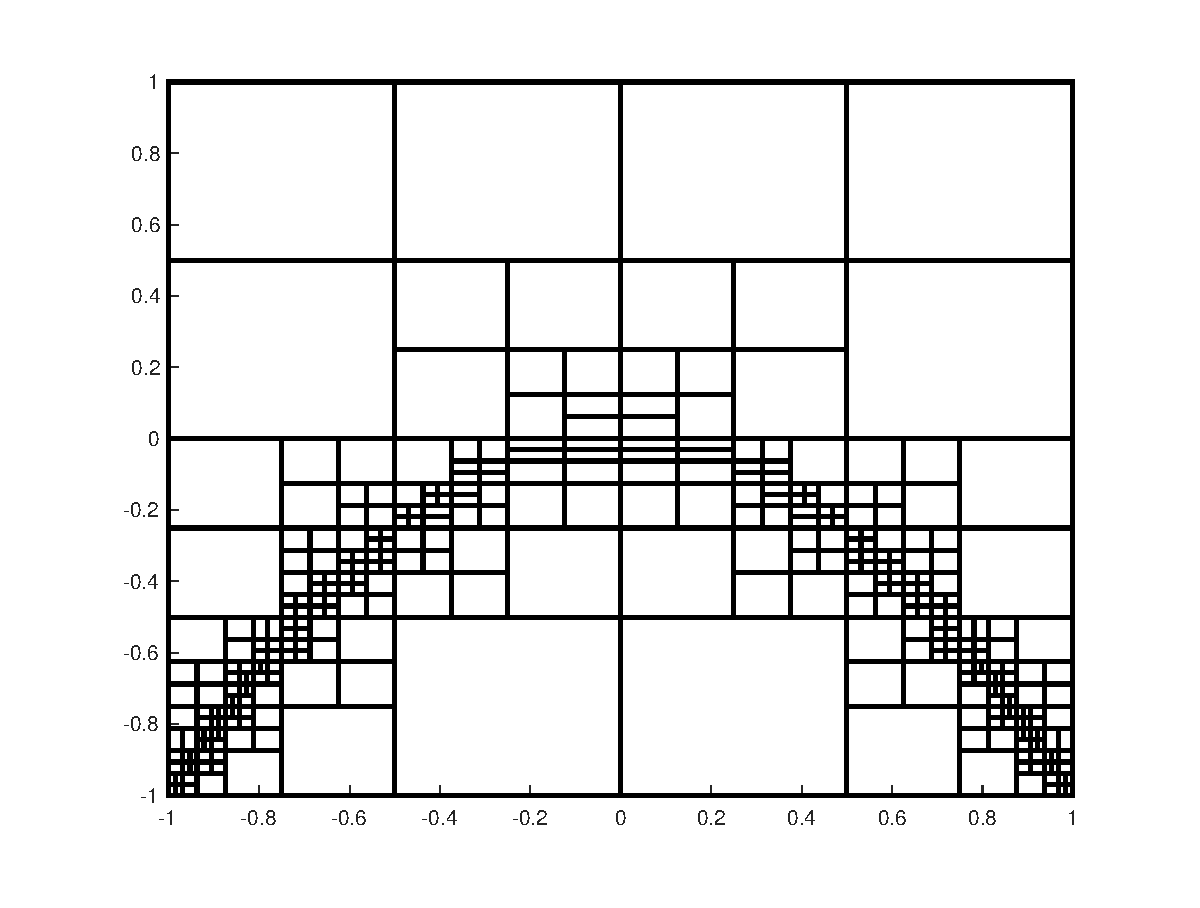
\includegraphics[scale = 0.3]{tan_100_1.eps}
   \label{zone_tan_a}
 }
\subfloat[Zone plot of $f_2(x,y)$]{
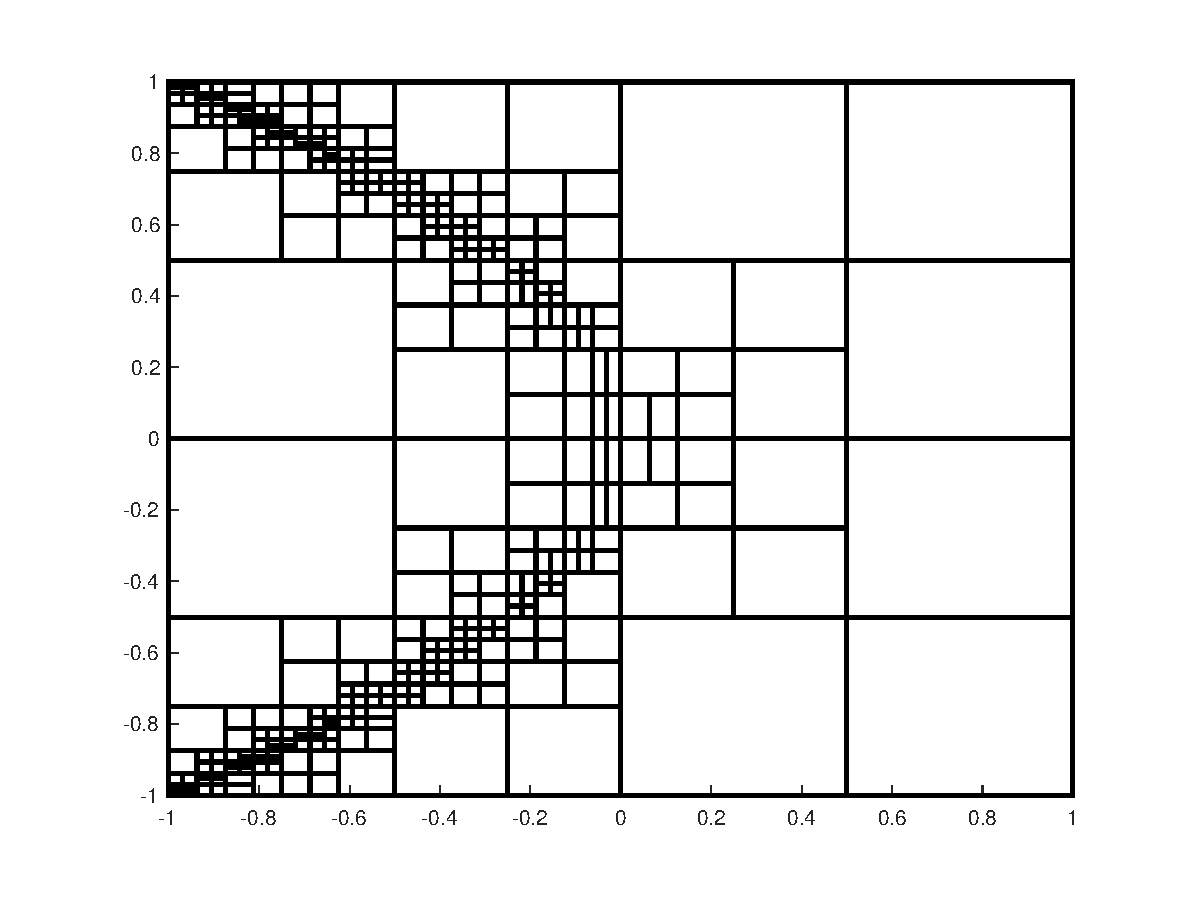
\includegraphics[scale = 0.3]{tan_100_2.eps}
   \label{zone_tan_b}
 }
 
 \subfloat[Zone plot of $f_1(x,y)+f_2(x,y)$]{
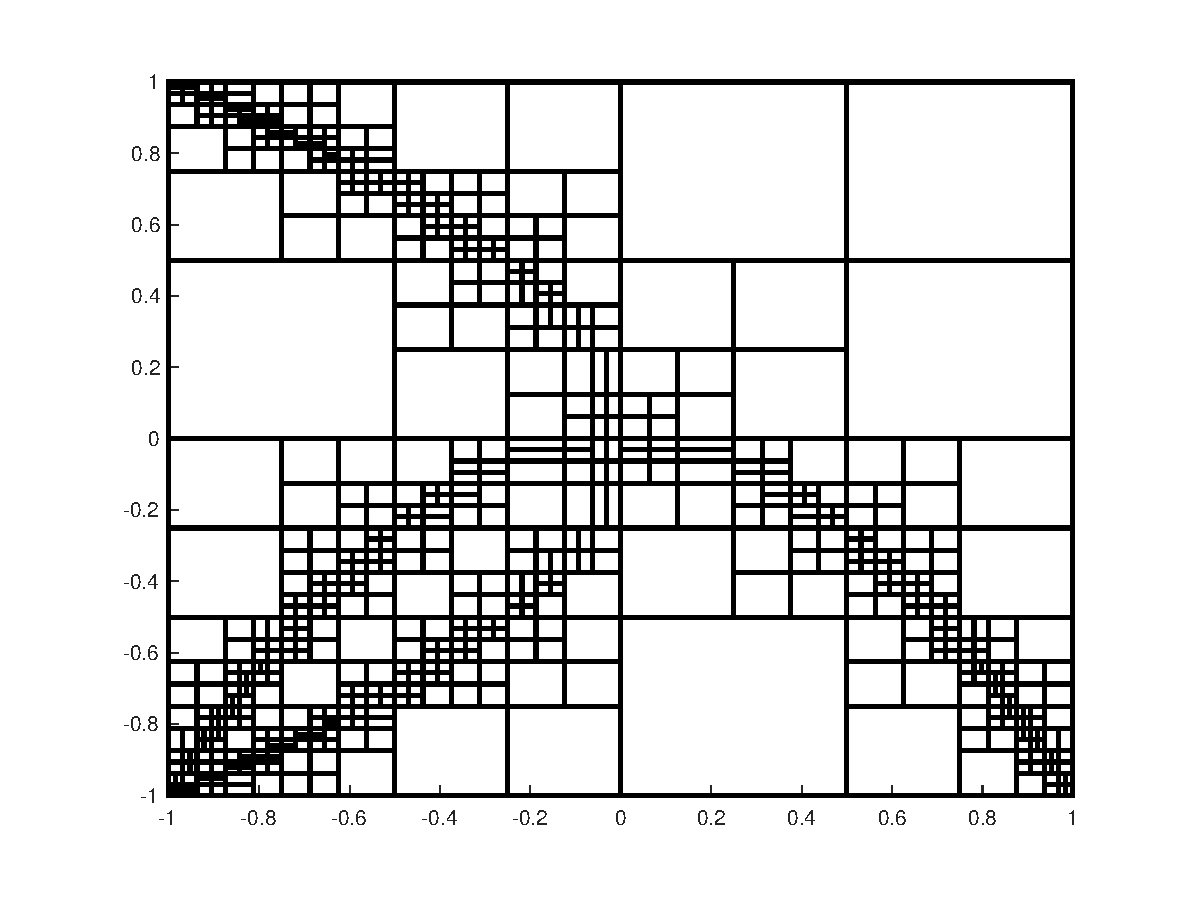
\includegraphics[scale = 0.3]{tan_100_3.eps}
   \label{zone_tan_c}
 }
 \caption{Zone plots for $f_1(x,y)$,$f_2(x,y)$ and $f_1(x,y)+f_2(x,y)$.}
\label{zone_tan}
\end{figure}
 

\subsection{Differentiation}
We compute partial derivatives of a PU approximation $s(\vect{x}) = \sum_{k=1}^m w_k(\vect{x}) s_k(\vect{x})$ patch by patch. For example if each $s_k(\vect{x})$ approximates $f(\vect{x})$, the the PU approximation of $\frac{\partial f(\vect{x})}{\partial x}$ we use is
\begin{equation}
	\frac{\partial f(\vect{x})}{\partial x} \approx \sum_{k=1}^m w_k(\vect{x})\frac{\partial s_k(\vect{x})}{\partial x}.
	\label{PU_diff} 
\end{equation}
Here it is important that each $\frac{\partial s_k(\vect{x})}{\partial x}$ approximates $\frac{\partial f(\vect{x})}{\partial x}$ locally since (\ref{PU_diff}) is not the derivative of the PU approximation itself.

\subsection{Integration}
With our method, the simplest approach for integration is to do so along the zones of the patches (that is, the non-overlapping domains). This is because for a set of patches $\{ \nu_k \}_{k=1}^{M}$
\begin{equation}
\int_{D} f(\vect{x}) d\vect{x} = \sum_{k=1}^{M} \int_{\text{\textsf{zone}($\nu_k$)}} f(\vect{x}) d\vect{x}.
\end{equation}
Thus if we have approximations respective approximations $\{ s_k(\vect{x}) \}_{k=1}^{M}$ for the patches, then
\begin{equation}
\int_{D} f(\vect{x}) d\vect{x} \approx \sum_{k=1}^{M} \int_{\text{\textsf{zone}($\nu_k$)}} s_k(\vect{x}) d\vect{x}.
\end{equation}
For each $s_k(\vect{x})$, we interpolate the approximation to a Chebyshev grid on \textsf{zone}($\nu_k$) and use Clenshaw-Curtis quadrature to approximate the local integrals \cite{mason2002chebyshev}.
\section{Numerical Experiments}
\label{numerical_experiments}

\subsection{2D experiments}
All our experiments were performed on a computer with a 2.6 GHz Intel core i5 processor in version 2017a of Matlab. We first test the 2D functions $\log(1+(x^2+y^4)/10^{-5})$, $\arctan((x+y^2)/10^{-2})$, $\frac{10^{-4}}{(10^{-4}+x^2)(10^{-4}+y^2)}$, Franke's function \cite{franke1979critical}, and the smooth functions from the Genz family test package \cite{genz1987package}. For each function we record the time of construction, the time to evaluate on a 200x200 grid, and the max error on this grid. 


Table~\ref{putable} shows the results for the adaptive PU method. For comparison, Table~\ref{chb2table} shows the results for Chebfun 2 \cite{townsend2013extension}, using version 5.5.0 of Chebfun. For the low-rank test cases, the methods are comparable, with neither showing a consistent advantage; most importantly, both methods are fast. In the tests of high-rank functions, the adaptive PU method enjoys a clear advantage in both construction and evaluation times. Moreover, the method remains fast enough for interactive computing even as the total number of nodes exceeds 1.6 million.  We include plots of the functions and adaptively generated subdomains for the first three test functions in Figures~\ref{TANFUN1}-\ref{rungeFUN1}.

As a simple experiment, we examine how the construction time changes with respect to rotation. We use the function
\begin{equation}
f(x,y)=\arctan(250(\cos(t)x+\sin(t)y))
\label{rotate_func_2D}	
\end{equation}
for $t \in [0,\pi/4]$. We plot the results in Figure~\ref{tan_rotate_2D}. As we rotate the interface, we would expect the numerical rank of $f(x,y)$ to increase as $t \to \pi/4$; this is observed in the time increase of the Chebfun2 construction in Figure~\ref{tan_rotate_2D}. The construction for the PU method however remains relatively constant despite the rotation.

We preform a similar experiment, but record the time to add and multiply $\arctan(250x)$ with (\ref{rotate_func_2D}) for $t \in [0,\pi/2]$, the results of which can be seen in Figure~\ref{TAN_ADD_MULT}. We first observe that the time to combine different PU approximations does not heavily depend on how the splittings of the different approximations align (we expect the splittings of $f(x,y)$ and $g(x,y)$ to differ as we rotate $f(x,y)$). We also see that the PU method out preforms except in cases where the sum or product is a low rank approximation itself.


\begin{table}[!htb]

\begin{tabular}{r|c|c|c|c}
& error & construct time & interp time & points \\[5pt] \hline
$\log(1+\frac{x_1^2+x_2^4}{10^{-5}})$ & 1.05e-13 & 0.6403 & 0.063 & 110496 \\[5pt]
$\arctan(\frac{x_1+x_2^2}{10^{-2}})$ & 2.15e-12 & 2.9690 & 0.3138 & 1553816 \\[5pt]
$\frac{10^{-4}}{(10^{-4}+x_1^2)(10^{-4}+x_2^2)}$ & 1.01e-11 & 0.7298 & 0.1087 & 145280 \\[2pt]
franke & 4.22E-15 & 0.0116 & 0.0045 & 16641 \\[2pt]
$\cos(u_1\pi + \sum_{i=1}^2 a_i x_i)$ & 2.65e-14 & 0.0127 & 0.0025 & 1089 \\[5pt]
$\prod_{i=1}^2 (a_i^{-2}+(x_i-u_i)^2)^{-1}$ & 5.00e-12 & 0.0555 & 0.016 & 29283 \\[2pt]
$(1+\sum_{i=1}^2 a_i x_i)^{-3}$ & 2.27e-12 & 0.0119 & 8.97e-04 & 25 \\[5pt]
$\exp(-\sum_{i=1}^2 a_i^2 (x_i-u_i)^2)$ & 1.65E-14 & 0.0130 & 0.0026 & 2145 \\
\end{tabular}
\caption{Table for our method tested with a 200x200 grid with recorded error, construction time, time to interpolate, and number of interpolation points used for the method. Here the target tolerance is set to $10^{-12}$, and $\nmax=129$. Here $u=[0.75,0.25]$, $a=[5,10]$.}
\label{putable}
\end{table}

\begin{figure}[!htb]
\centering

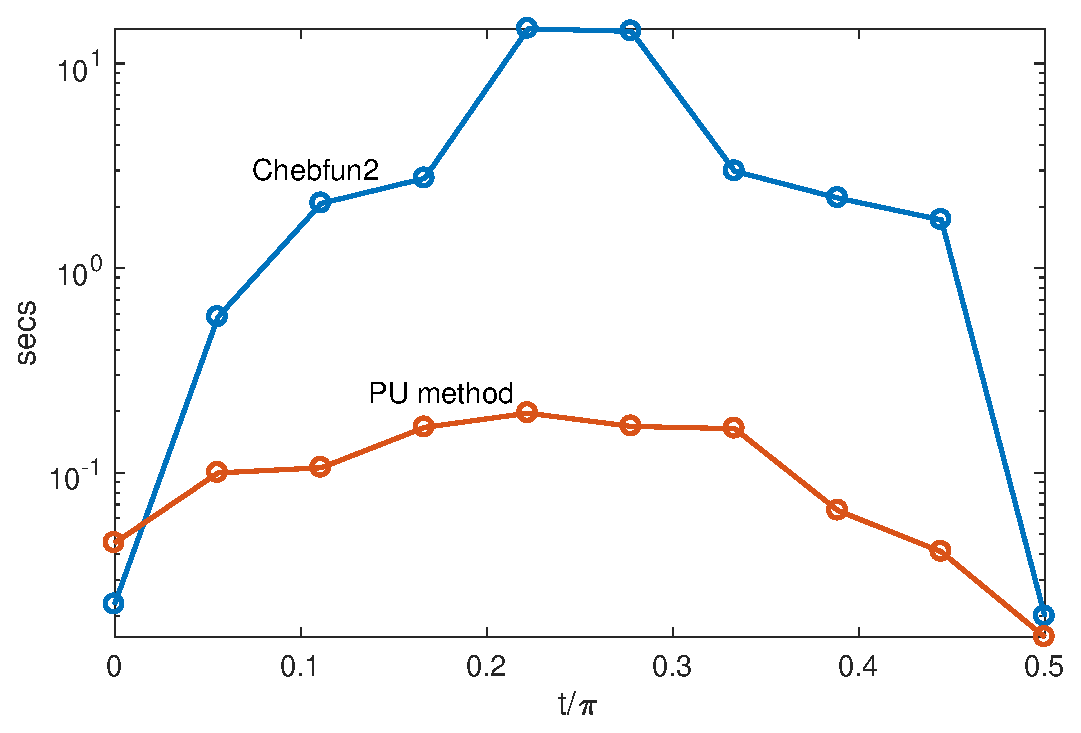
\includegraphics[scale = 0.5]{tan_rotatate_2D.eps}

\caption{Plot of construction time of $\arctan(250(\cos(t)x+\sin(t)y))$ for $t \in [0,\pi/4]$ for the partition of unity method and Chebfun2.}
\label{tan_rotate_2D}
\end{figure}




\begin{figure}[!htbp]
\centering
\subfloat[Plot of $\arctan \lp (x+y^2)/0.01 \rp$.]{
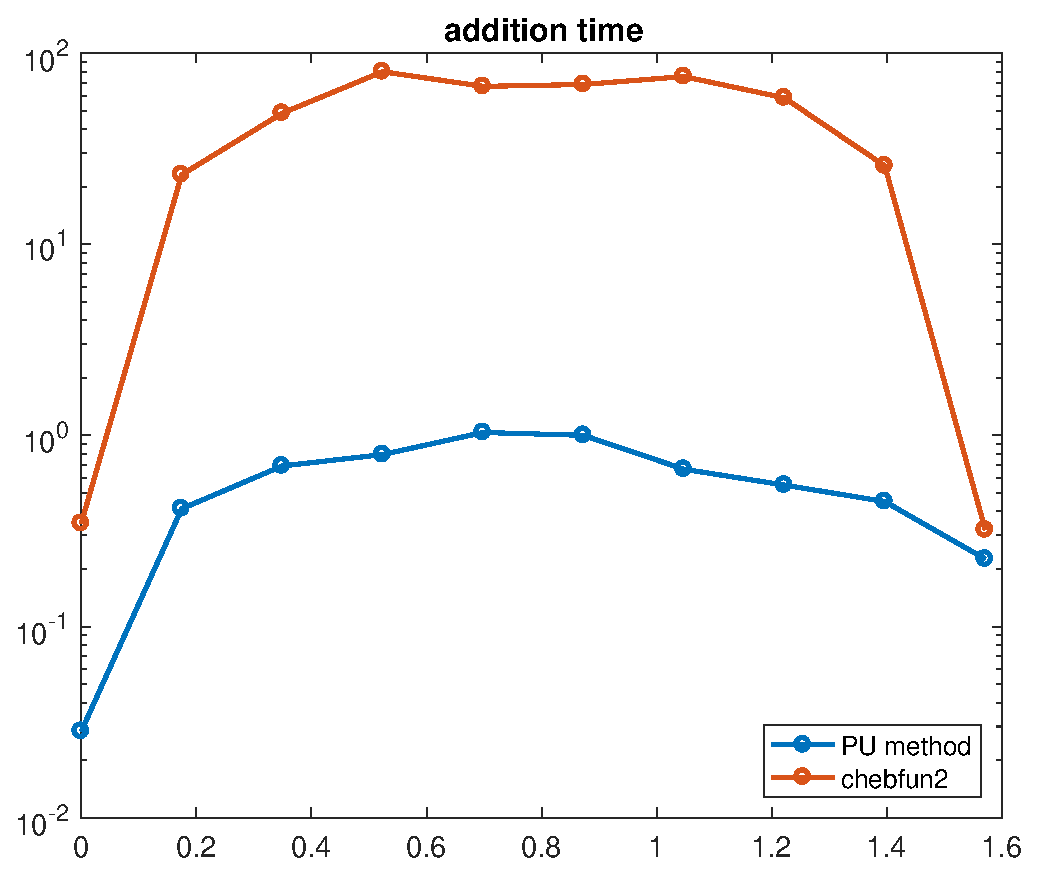
\includegraphics[scale = 0.34]{tan_add2D_1.eps}
   \label{add_plot_1}
 }
\subfloat[Plot of subdomains.]{
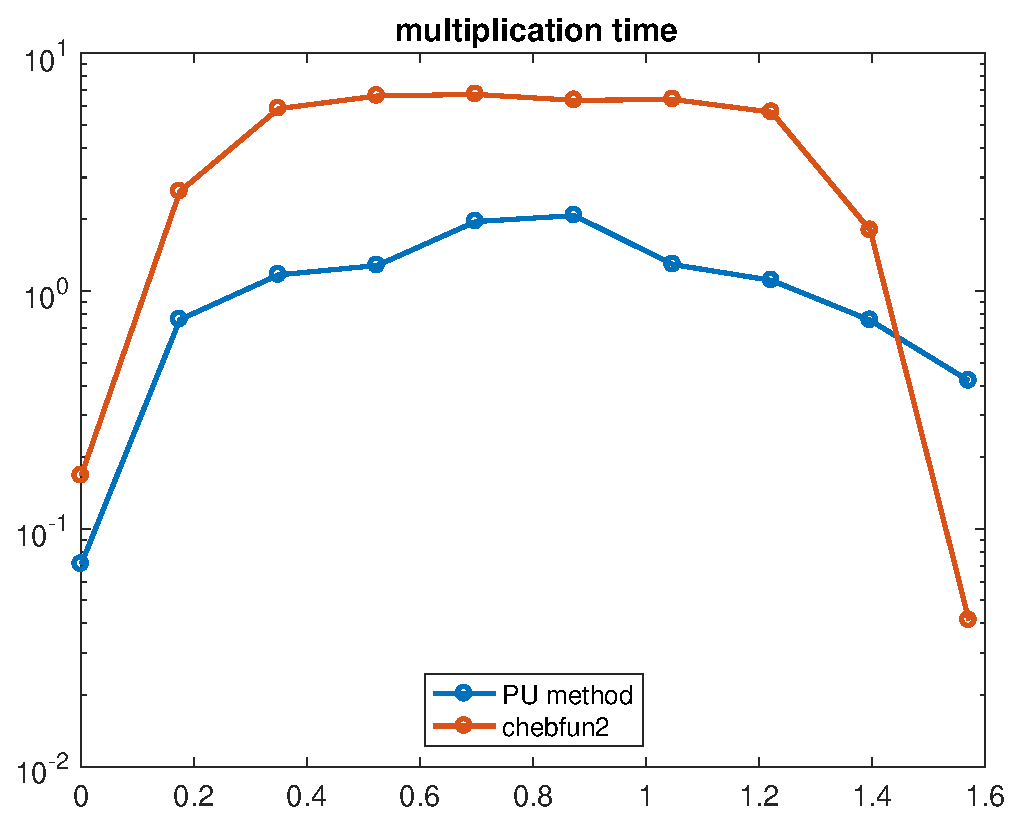
\includegraphics[scale = 0.34]{tan_mult2D_1.eps}
   \label{mult_plot_1}
 }
\caption{Plot of $\arctan \lp (x+y^2)/0.01 \rp$ and the subdomains formed from the partition of unity method.}
\label{TAN_ADD_MULT}
\end{figure}

\begin{table}[!htb]
\begin{tabular}{r|c|c|c|c}
& obsd error & time & interp time & rank \\[5pt] \hline
$\log(1+\frac{x_1^2+x_2^4}{10^{-5}})$ & 1.14E-06 & 2.2997 & 0.1045 & 30 \\[5pt]
$\arctan(\frac{x_1+x_2^2}{10^{-2}})$ & 7.09E-12 & 150.2228 & 4.979 & 816 \\[5pt]
$\frac{10^{-4}}{(10^{-4}+x_1^2)(10^{-4}+x_2^2)}$ & 5.44E-15 & 0.0493 & 0.0037 & 1 \\[5pt]
franke & 1.33E-15 & 0.0198 & 0.0024 & 4 \\[5pt]
$\cos(u_1\pi + \sum_{i=1}^2 a_i x_i)$ & 4.47E-14 & 0.0155 & 0.002 & 2 \\[5pt]
$\prod_{i=1}^2 (a_i^{-2}+(x_i-u_i)^2)^{-1}$ & 1.59E-12 & 0.0203 & 0.0022 & 1 \\[5pt]
$(1+\sum_{i=1}^2 a_i x_i)^{-3}$ & 2.27E-12 & 0.0117 & 0.0021 & 4 \\[5pt]
$\exp(-\sum_{i=1}^2 a_i^2 (x_i-u_i)^2)$ & 4.44E-16 & 0.0149 & 0.0022 & 1 \\[5pt]
\end{tabular}
\caption{Table for Chebfun2 tested with a 200x200 grid with recorded error, construction time, time to interpolate, and numerical rank. Here the target tolerance is set to $10^{-12}$, and $\nmax=129$. Here $u=[0.75,0.25]$, $a=[5,10]$.}	
\label{chb2table}
\end{table}


\begin{figure}[!htbp]
\centering
\subfloat[Plot of $\arctan \lp (x+y^2)/0.01 \rp$.]{
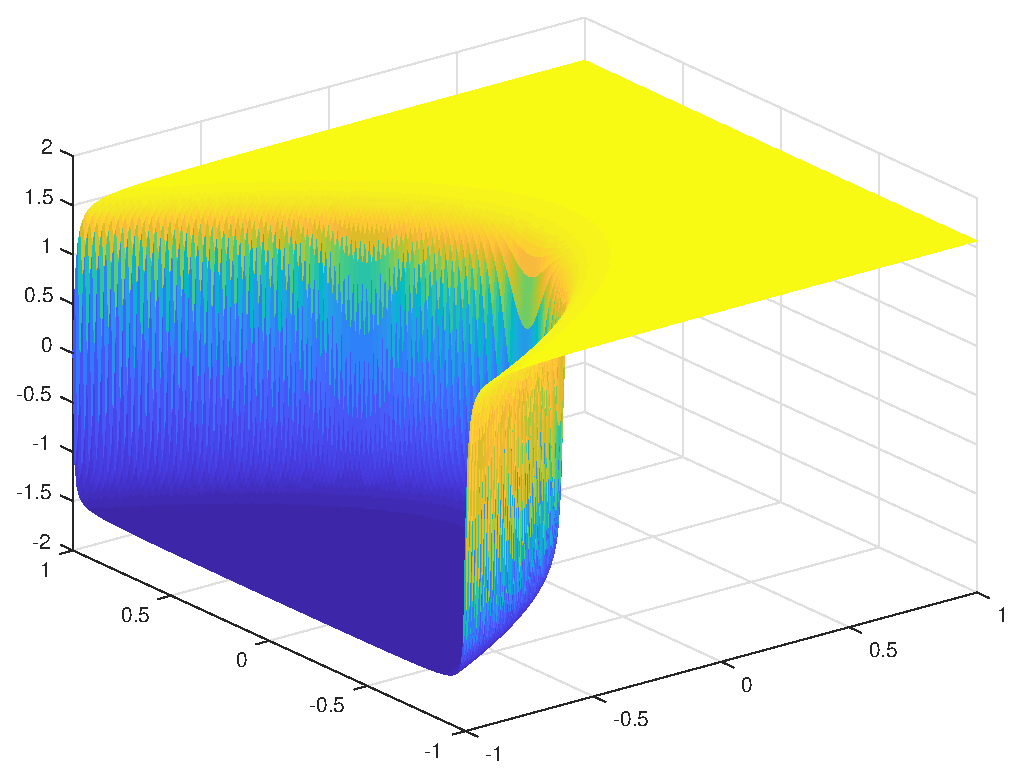
\includegraphics[scale = 0.34]{tan2Dplot.eps}
   \label{tanfunplot}
 }
\subfloat[Plot of subdomains.]{
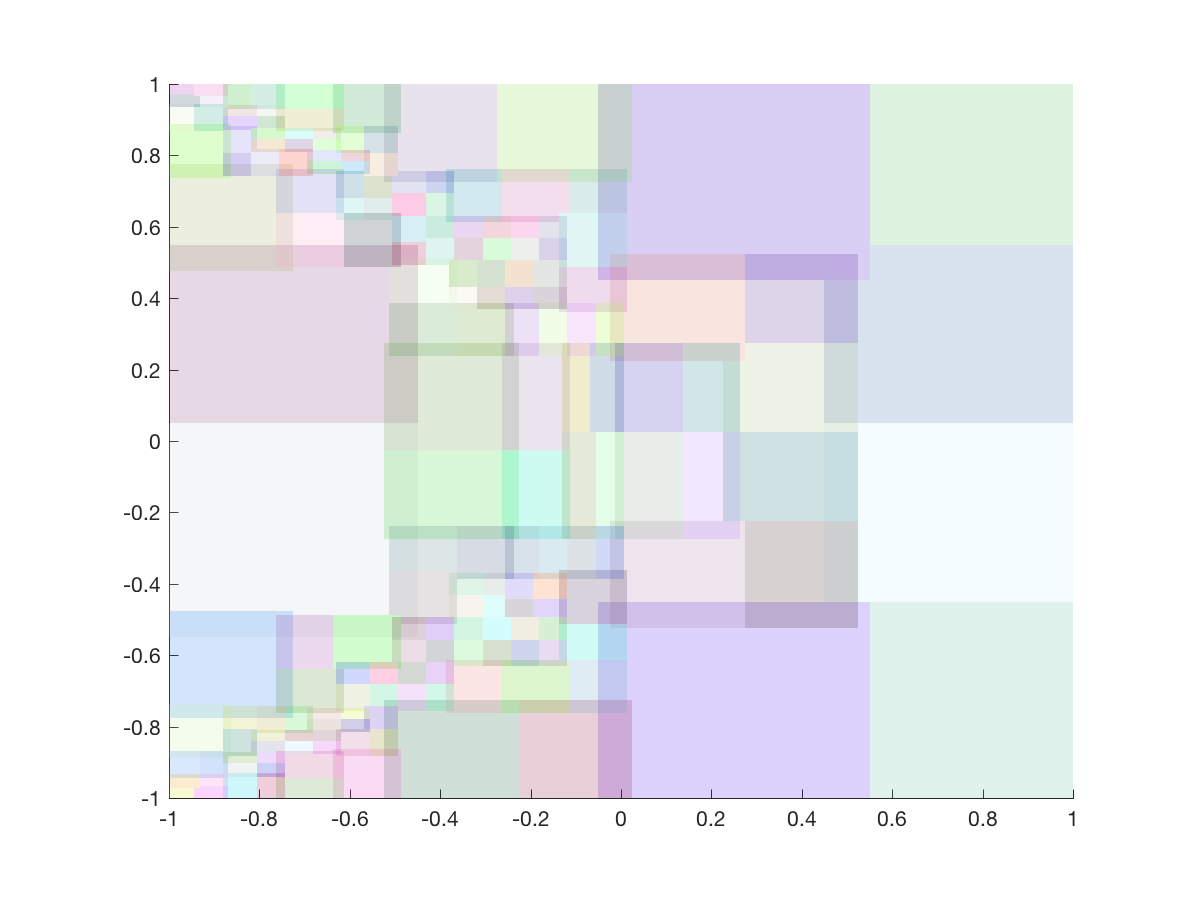
\includegraphics[scale = 0.34]{tan2Dsubdomains.eps}
   \label{tanfundomains}
 }
\caption{Plot of $\arctan \lp (x+y^2)/0.01 \rp$ and the subdomains formed from the partition of unity method.}
\label{TANFUN1}
\end{figure}

\begin{figure}[!htbp]
\centering
\subfloat[Plot of $\log(1+(x^2+y^4)/10^{-5})$.]{
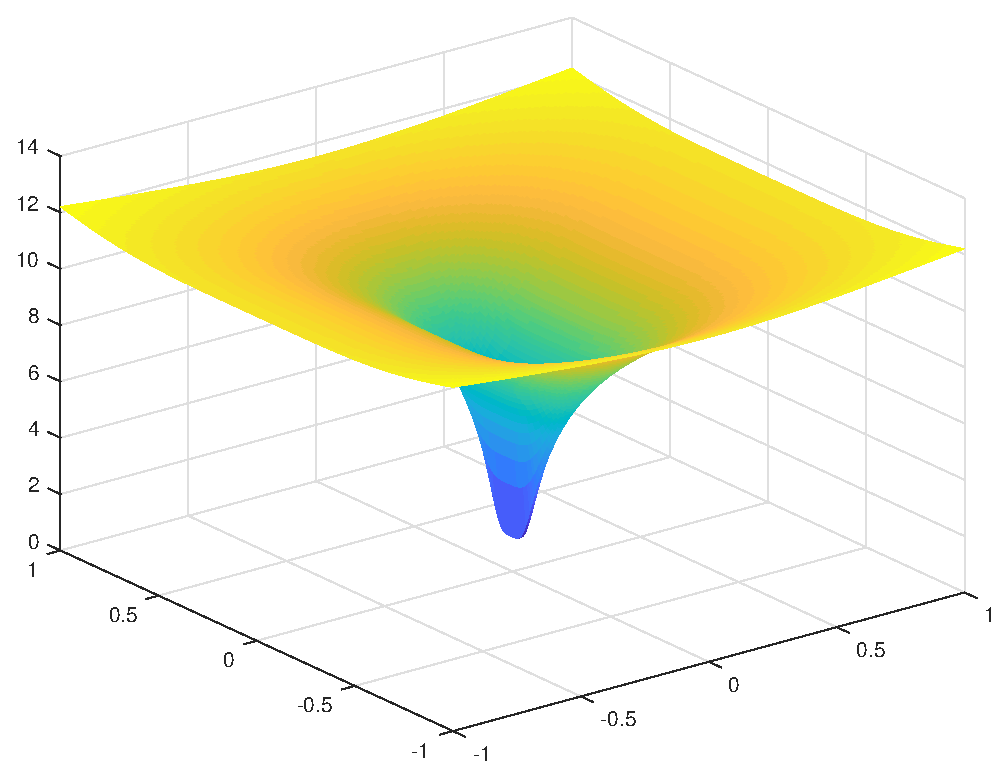
\includegraphics[scale = 0.34]{log2Dplot.eps}
   \label{logfunplot}
 }
\subfloat[Plot of subdomains.]{
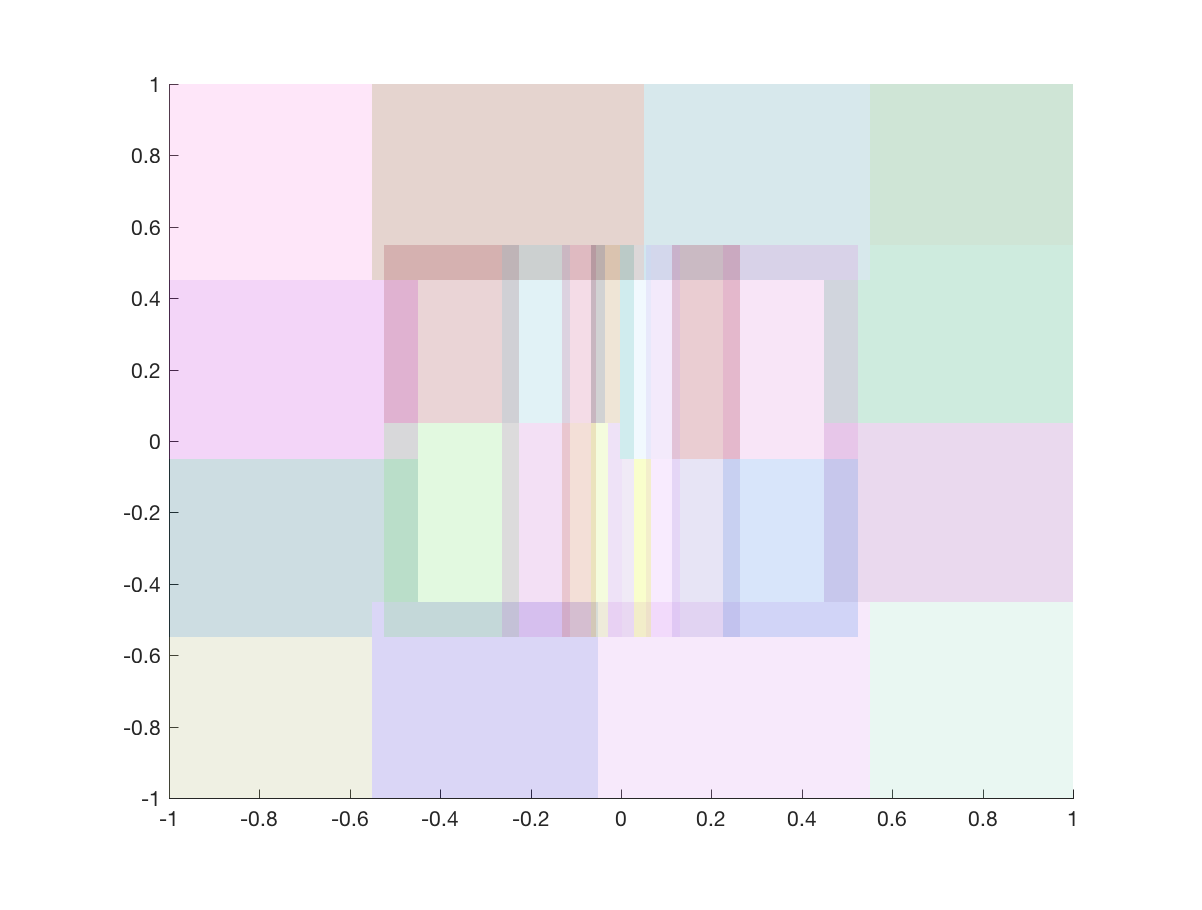
\includegraphics[scale = 0.34]{log2Dsubdomains.eps}
   \label{logfundomains}
 }
\caption{Plot of $\log(1+(x^2+y^4)/10^{-5})$ and the subdomains formed from the partition of unity method.}
\label{logFUN1}
\end{figure}

\begin{figure}[!htbp]
\centering
\subfloat[Plot of $\frac{10^{-4}}{(10^{-4}+x^2)(10^{-4}+y^2)}$.]{
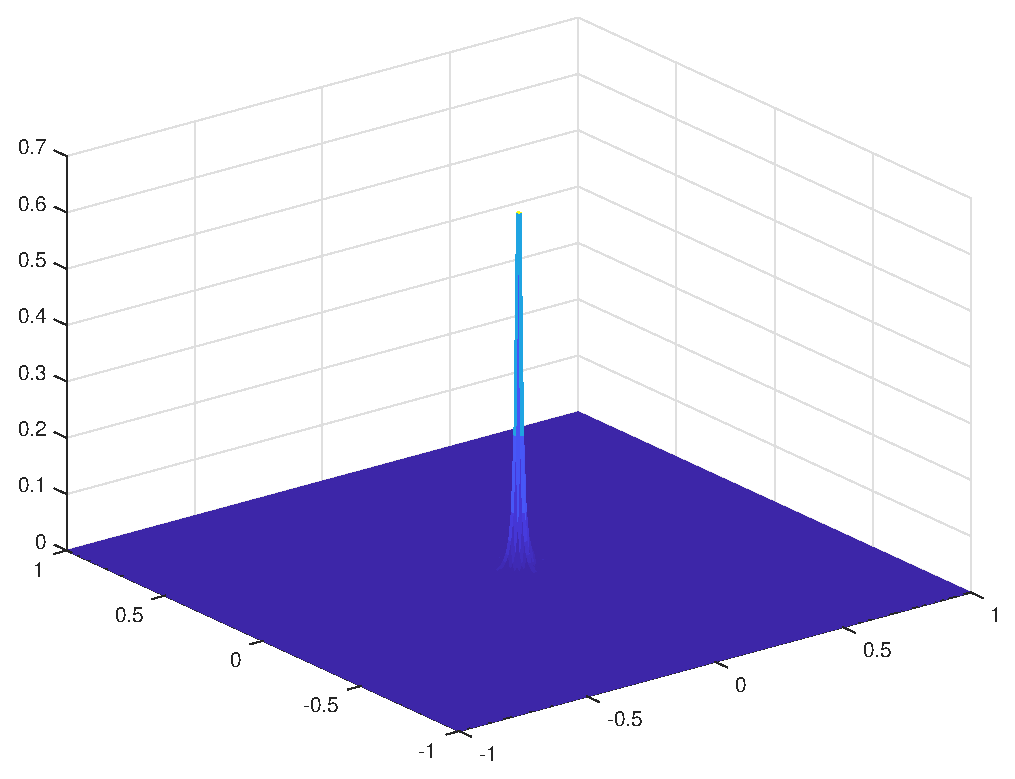
\includegraphics[scale = 0.34]{runge2Dplot.eps}
   \label{rungefunplot}
 }
\subfloat[Plot of subdomains.]{
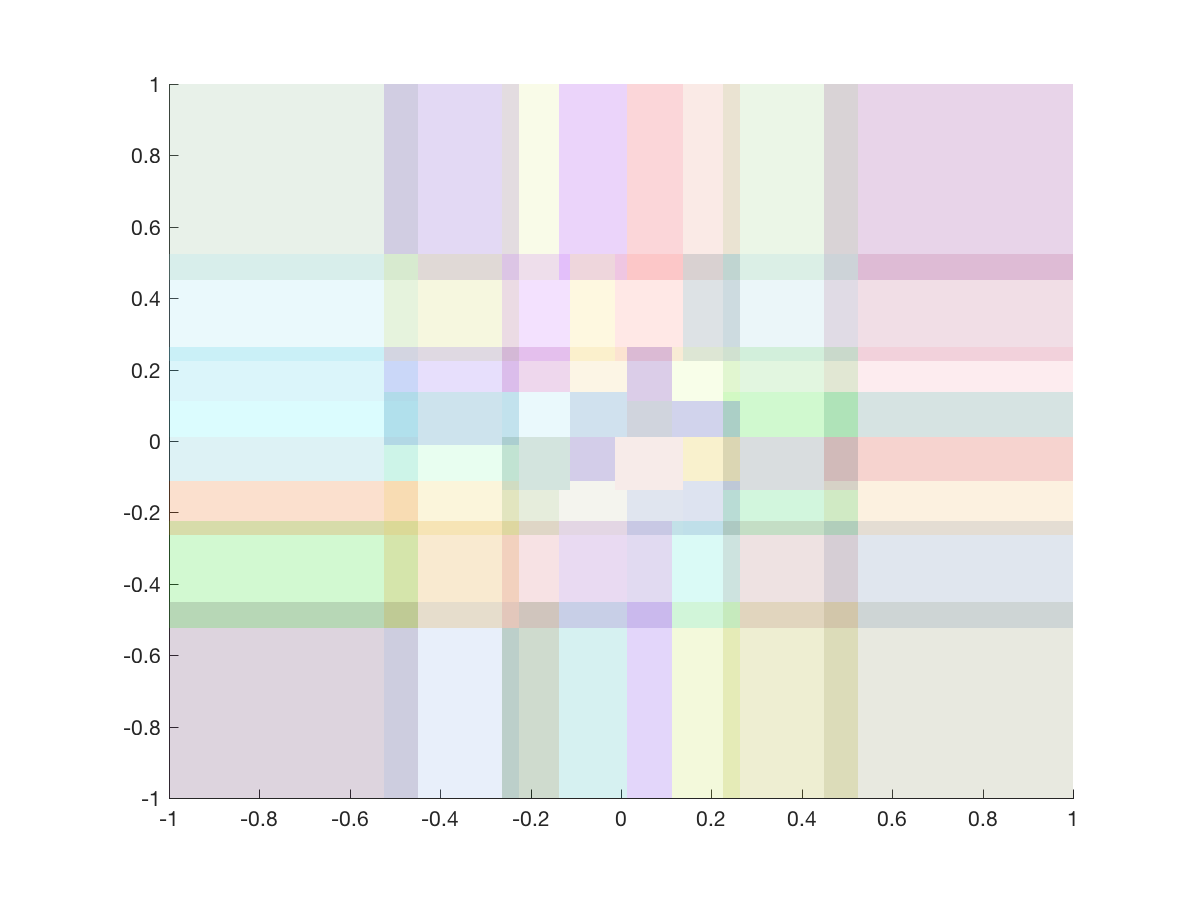
\includegraphics[scale = 0.34]{rungesubdomains.eps}
   \label{rungefundomains}
 }
\caption{Plot of $\frac{10^{-4}}{(10^{-4}+x^2)(10^{-4}+y^2)}$ and the subdomains formed from the partition of unity method.}
\label{rungeFUN1}
\end{figure}

\subsection{3D experiments} We next test the 3D functions $1/(\cosh(5(x+y+z)))^2$, $\arctan(5(x+y)+z)$ and the smooth functions from the Genz family test package again, but in 3D. We similarly record the construction time, time to evaluate on a $200\times 200 \times 200$ grid and the max error on the grid.

We have the results for the PU method and Chebfun3 \cite{hashemi2017chebfun} in Tables~\ref{putable3D},\ref{chb3table}. We see that Chebfun3 preforms well for low rank functions \footnote{In Chebfun3, functions are approximated in a compressed splice-Tucker decomposition, a variant of a multivariate adaptive cross approximation \cite{bebendorf2011adaptive}. Here the rank refers to the so called tucker rank. }, and out preforms when there are sharp singularities as seen with the Genz function with the Runge singularities. For high rank functions there is an evident advantage in construction times, and evaluation times are comparable. For $\arctan(5(x+y)+z)$ we see a dramatic difference in the construction time; this is because the PU method stops splitting in the $z$-direction early as seen in Figure~\ref{tan_not_z}.

We preform a rotation experiment with the function
\begin{equation}
\arctan(5(\sin(p)\cos(t)x+\sin(p)\sin(t)y+\cos(p)z))
\end{equation}
for $p,t \in [0,\pi/4]$ where we record the construction time for our method and Chebfun3. The results can be seen in Figure~\ref{tan3D}. We see that slight changes in $t,p$ can dramatically increase the construction time, where rotations have a slight effect with the PU method.

\begin{figure}[!htbp]
\centering
\subfloat[PU method]{
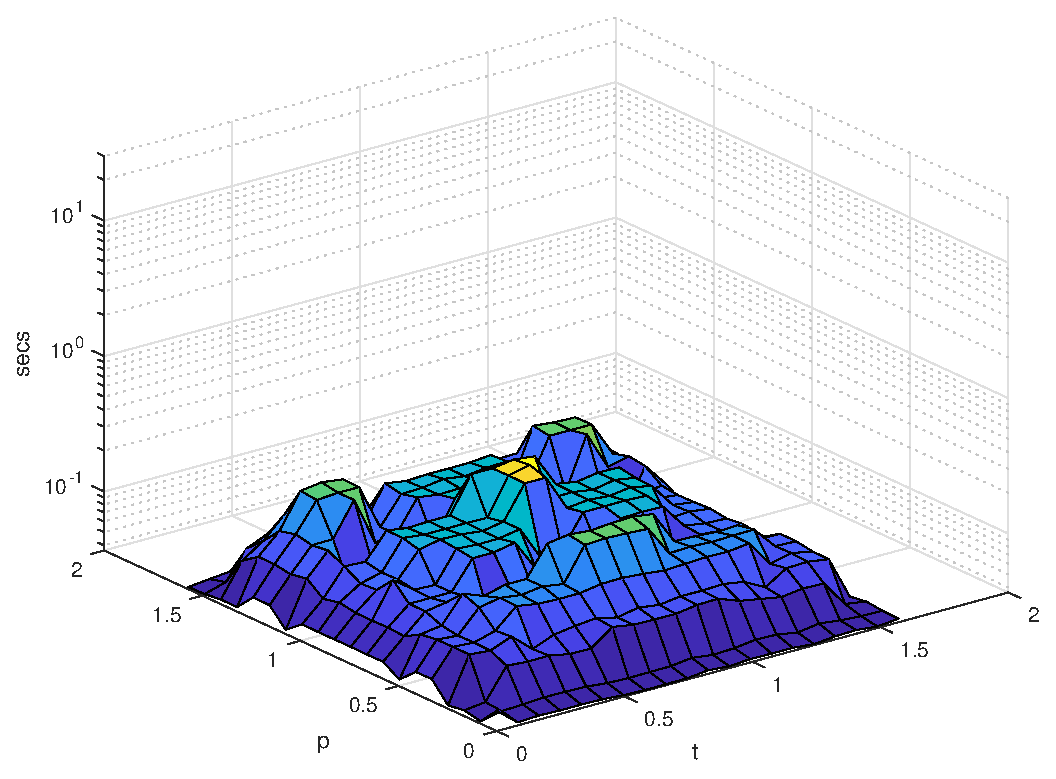
\includegraphics[scale = 0.34]{TAN_3D_PU.eps}
   \label{tan3DPU}
 }
\subfloat[Chebfun3]{
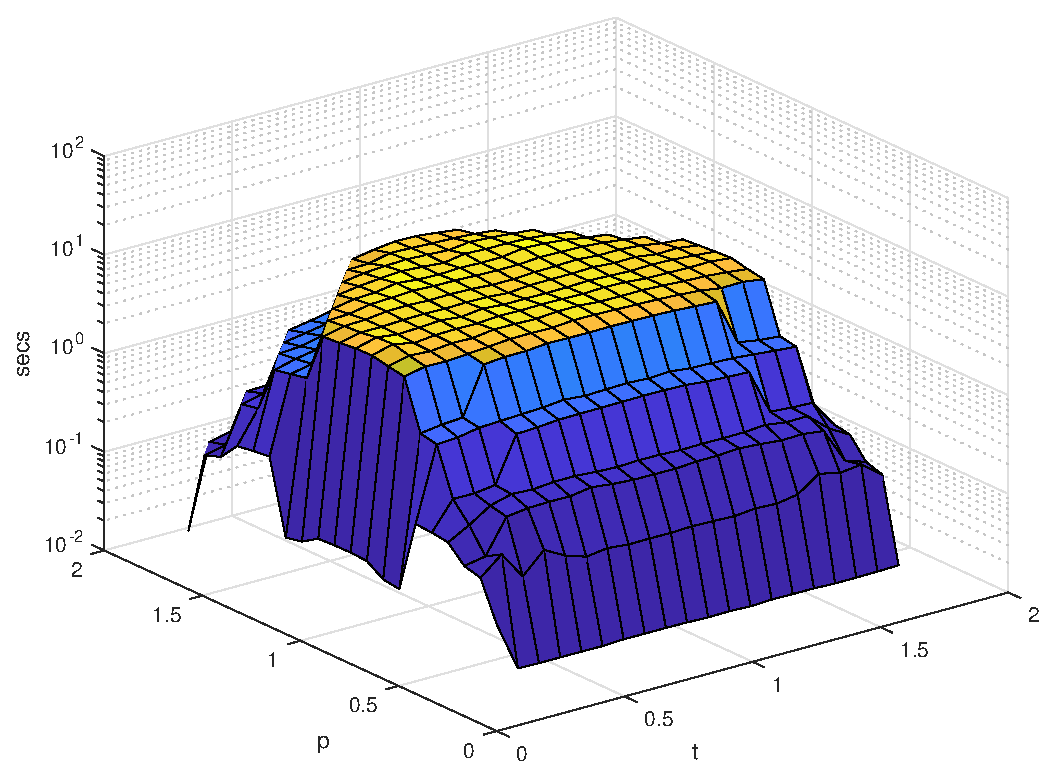
\includegraphics[scale = 0.34]{TAN_3D_CHEB.eps}
   \label{tan3DCheb}
 }
\caption{Plot of construction time of $\arctan(5(\sin(p)\cos(t)x+\sin(p)\sin(t)y+\cos(p)z))$ for $t,p \in [0,\pi/4]$ for the PU method and Chebfun3.}
\label{tan3D}
\end{figure}



\begin{table}
\begin{tabular}{r|c|c|c|c}
& error & construct time & interp time & points \\[5pt] \hline
$\cos(u_1\pi + \sum_{i=1}^3 a_i x_i)$ & 22.71E-14 & 0.151 & 0.118 & 275000 \\ [5pt]
$\prod_{i=1}^3 (a_i^{-2}+(x_i-u_i)^2)^{-1}$ & 1.52E-05 & 7.204 & 1.312 & 10400000 \\[2pt]
$(1+\sum_{i=1}^3 a_i x_i)^{-3}$ & 4.66E-10 & 0.16555 & 0.033 & 125 \\[5pt]
$\exp(-\sum_{i=1}^2 a_i^2 (x_i-u_i)^2)$ & 3.11E-15 & 0.0818 & 0.078 & 275000  \\[5pt]
$1/(\cosh(5(x+y+z)))^2$ & 1.14E-14 & 0.706 & 0.545 & 2200000 \\
$\arctan(5(x+y)+z)$ & 7.60e-13 & 0.7512 & 0.030 & 549153 \\
\end{tabular}
\caption{Table for our method tested with a $200^3$ grid with recorded error, construction time, time to interpolate, and number of interpolation points used for the method. Here the target tolerance is set to $10^{-12}$, and $\nmax=65$. Here $u=[0.75,0.25,-0.75]$, $a=[25,25,25]$.}
\label{putable3D}
\end{table}

\begin{table}
\begin{tabular}{r|c|c|c|c}
& error & construct time & interp time & rank \\[5pt] \hline
$\cos(u_1\pi + \sum_{i=1}^2 a_i x_i)$ & 2.16E-14 & 0.061 & 0.150 & 2  \\[5pt]
$\prod_{i=1}^2 (a_i^{-2}+(x_i-u_i)^2)^{-1}$ & 5.66E-07 & 0.057 & 0.137 & 1 \\[5pt]
$(1+\sum_{i=1}^2 a_i x_i)^{-3}$ & 4.07E-10 & 0.038 & 0.143 & 4 \\[5pt]
$\exp(-\sum_{i=1}^2 a_i^2 (x_i-u_i)^2)$ & 7.77E-16 & 0.047 & 0.144 & 1 \\[5pt]
$1/(\cosh(5(x+y+z)))^2$ & 3.69E-13 & 80.666 & 0.398 & 93 \\
$\arctan(5(x+y)+z)$ & 4.69e-13 & 89.957 & 0.104 & 110 \\
\end{tabular}
\caption{Table for Chebfun3 tested with a $200^3$ grid with recorded error, construction time, time to interpolate, and numerical rank. Here $u=[0.75,0.25,-0.75]$, $a=[25,25,25]$.}	
\label{chb3table}
\end{table}

\begin{figure}[!htb]
\centering

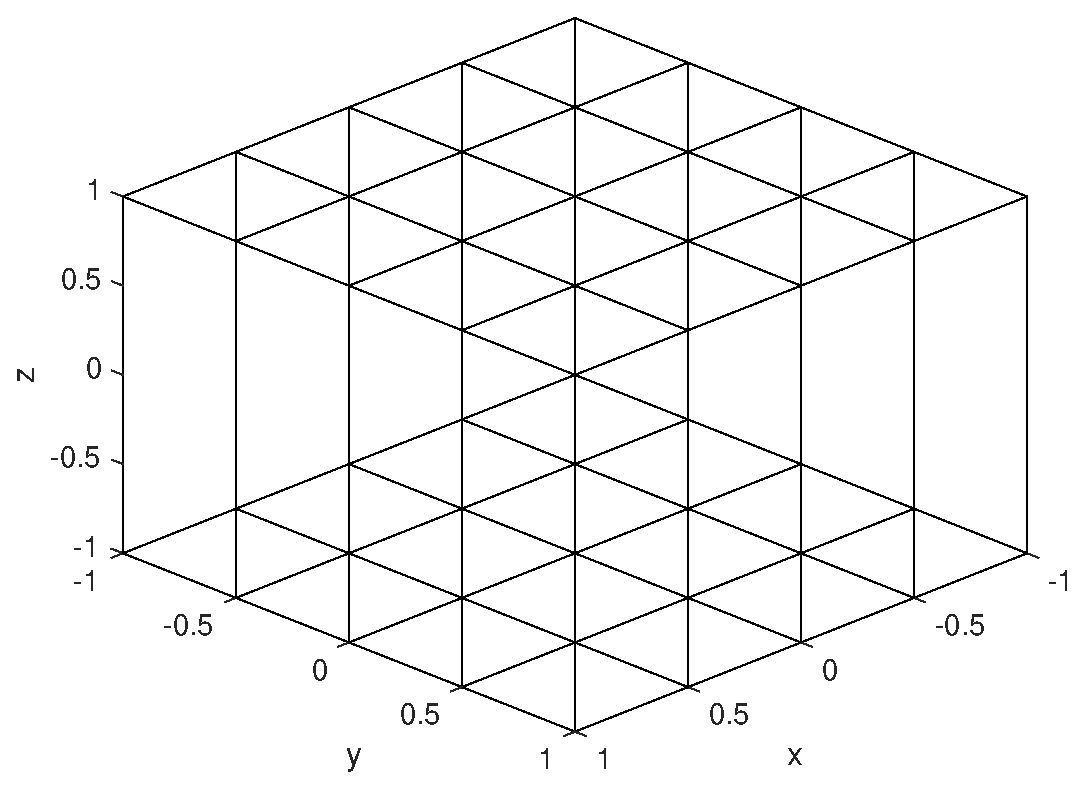
\includegraphics[scale = 0.5]{tan_not_z.eps}

\caption{Plot of zones for $\arctan(5(x+y)+z)$.}
\label{tan_not_z}
\end{figure}

\begin{appendices}

\section{Merging trees}
\label{sec:merge}

\newcommand{\Tm}{\ensuremath{\nu_\text{merge}}}
Algorithm~\ref{alg:merge} describes a recursive method for merging two trees $T_1$ and $T_2$, representing functions $f_1$ and $f_2$, into a tree representation for $f_1\circ f_2$, with $\circ$ as $+$, $-$, $\times$, or $\div$. The input arguments to the algorithm are the operation, corresponding nodes of $T_1$, $T_2$, and the merged tree, and the number $r$, which is the dimension that was most recently split in the merged tree. Initially the algorithm is called with root nodes representing the entire original domain, and $r=0$. 

We assume an important relationship among the input nodes. Suppose that \prop{zone}{$\nu_k$}=$\prod_{j=1}^d [\alpha_{kj},\beta_{kj}]$ for $k=1,2$, and that \prop{zone}{$\Tm$}=$\prod_{j=1}^d [A_{j},B_{j}]$. Then we require for $k=1,2$ that
\begin{equation}
  \label{eq:merge-zones}
  [a_{kj},b_{kj}]=[A_j,B_j] \quad \text{for all $j$ having} \quad   \prop{isdone}{\nu_k}_j=
  \text{FALSE}.
\end{equation}
This is trivially true at the root level. The significance of this requirement is that it allows us to avoid ambiguity about what the zone of $\Tm$ should be after a new split in, say, dimension $j$. Since only an uncompleted dimension can be split, the zone of the children of \Tm after splitting will be identical to that of whichever (or both) of the $\nu_k$ requires refinement in dimension $j$.

For example, suppose the zones of $\nu_1$ and $\nu_2$ are $[-1,0]\times[-1,1]$ and $[-1,1]\times[0,1]$, respectively, and \prop{zone}{\Tm}=$[-1,0]\times[0,1]$. It's clear that we can interpolate from $\nu_1$ and $\nu_2$ onto \Tm. It's also clear that we can further split in $x$ in $\nu_1$, and in $y$ in $\nu_2$. But if we were to split $\nu_2$ in $x$, one of the children would have zone $[0,1]\times[0,1]$, which is inaccessible to $\nu_1$. 

Consider the general recursive call. If both $\nu_1$ and $\nu_2$ are leaves, then we simply evaluate the result of operating on their interpolants to get the values on \Tm. If exactly one of $\nu_1$ and $\nu_2$ is a leaf, then we split \Tm the same way as the non-leaf and recurse into the resulting children; property~(\ref{eq:merge-zones}) trivially remains true in these calls. If both  $\nu_1$ and $\nu_2$ are non-leaves, and they both split in the same dimension, then we can split $\Tm$ in that dimension and recurse, and the zones will continue to match as in~(\ref{eq:merge-zones}).

The only remaining case is that $\nu_1$ and $\nu_2$ are each split, but in different dimensions. In this case we have to use information about how the splittings are constructed in Algorithm~\ref{alg:splitleaves}. Recall that each unresolved dimension is split in order, while resolved dimensions are flagged as finished in all descendants. By inductive assumption, \Tm was most recently split in dimension $r$. The algorithm determines which $\nu_k$ has splitting dimension $j$ that comes the soonest after $r$ (computed cyclically). Thus for all dimensions between $r$ and $j$, neither of the given nodes splits, so it and its descendants all must have \textsf{isdone} set to TRUE in those dimensions, and property~(\ref{eq:merge-zones}) makes no requirement. Furthermore, the dimension $r_k$ does satisfy~(\ref{eq:merge-zones}) for $\nu_k$, and the same will be true for its children and the children of $\Tm$. All other dimensions will inherit~(\ref{eq:merge-zones}) from the parents. 


\newcommand{\op}{\ensuremath{\circ}}
\begin{algorithm}[!h]
\caption{merge(\op,$\nu_1$,$\nu_2$,$T_{\text{merge}}$,$r$)}
\label{alg:merge}
\begin{algorithmic}
\IF{$\nu_1$ and $\nu_2$ are leaves}
\STATE \textsf{values}($T_{\text{merge}}$):= \textsf{interpolant}($\nu_1$) $\op$ \textsf{interpolant}($\nu_2$), evaluated on \prop{grid}{$T_\text{merge}$}
\ELSIF{$\nu_1$ is a leaf \AND $\nu_2$ is not a leaf}
\STATE split($T_{\text{merge}}$,\prop{splitdim}{$\nu_1$})
\STATE merge(\op,$\nu_1$,\child{0}($\nu_2$),\child{0}($T_{\text{merge}}$),\prop{splitdim}{$\nu_2$})
\STATE merge(\op,$\nu_1$,\child{1}($\nu_2$),\child{1}($T_{\text{merge}}$),\prop{splitdim}{$\nu_2$})
\ELSIF{$\nu_1$ is not a leaf \AND $\nu_2$ is a leaf}
\STATE split($T_{\text{merge}}$,\prop{splitdim}{$\nu_1$})
\STATE merge(\child{0}($\nu_1$),$\nu_2$,\child{0}($T_{\text{merge}}$),\prop{splitdim}{$\nu_1$})
\STATE merge(\child{1}($\nu_1$),$\nu_2$,\child{1}($T_{\text{merge}}$),\prop{splitdim}{$\nu_1$})
\ELSE
\IF{\prop{splitdim}{$\nu_1$}=\prop{splitdim}{$\nu_2$}}
\STATE split($T_{\text{merge}}$,\prop{splitdim}{$\nu_1$})
\STATE merge(\op,\child{0}($\nu_1$),\child{0}($\nu_2$),\child{0}($T_{\text{merge}}$),\prop{splitdim}{$\nu_1$})
\STATE merge(\op,\child{1}($\nu_1$),\child{1}($\nu_2$),\child{1}($T_{\text{merge}}$),\prop{splitdim}{$\nu_1$})
\ELSE
\STATE $r_1 = (\text{\prop{splitdim}{$\nu_1$}}-r-1) \mod d$
\STATE $r_2 = (\text{\prop{splitdim}{$\nu_2$}}-r-1) \mod d$
\STATE If $r_1>r_2$, swap $\nu_1$ and $\nu_2$
\STATE split($T_{\text{merge}}$,\prop{splitdim}{$\nu_1$})
\STATE merge(\op,\child{0}($\nu_1$),$\nu_2$,\child{0}($T_{\text{merge}}$),\prop{splitdim}{$\nu_1$})
\STATE merge(\op,\child{1}($\nu_1$),$\nu_2$,\child{1}($T_{\text{merge}}$), \prop{splitdim}{$\nu_1$})
\ENDIF
\ENDIF
\end{algorithmic}
\end{algorithm}




%\begin{theorem}
%Algorithm~\ref{addition3} produces a tree $T_{\text{add}}$ with a merged splitting of $\nu_1$ and $\nu_2$.
%\label{split_theorem_2}
%\end{theorem}
%
%\begin{proof}
%Suppose we have that \textsf{zone}($T_{\text{add}}$) and \textsf{zone}($\nu_1$) are the same along the first dimension i.e. if \textsf{zone}($T_{\text{add}}$)=$[a,b]\times[c,d]$ and \textsf{zone}($\nu_1$)=$[e,f]\times[g,h]$ then $[a,b]=[e,f]$. Then it is clear that if $\nu_1$ and $T_{\text{add}}$ split first in $x$ that \textsf{zone}(\child{k}($T_{\text{add}}$)) and \textsf{zone}(\child{k}($\nu_1$)) will match along the first dimension as well. Suppose for induction that for $k=0,1$ \textsf{zone}($T_{\text{add}}$) and \textsf{zone}($T_k$) are the same along dimensions that $T_k$ still splits in. This is trivially true at the first call since at the root \textsf{zone}($T_{\text{add}}$)=\textsf{zone}($\nu_1$)=\textsf{zone}($\nu_2$).
%
%Suppose we are at a case where $\nu_1$ is not a leaf and we split \textsf{zone}($T_{\text{add}}$) along \textsf{splitdim}($\nu_1$). By the induction hypothesis we have that \textsf{zone}($T_{\text{add}}$) matches \textsf{zone}($\nu_1$) along dimension \textsf{splitdim}($\nu_1$); this gives us that \textsf{zone}(\child{k}($T_{\text{add}}$)) and \textsf{zone}(\child{k}($\nu_1$)) match along \textsf{splitdim}($\nu_1$) as well. Since nothing has changed for the other dimensions, the induction hypothesis holds for \child{k}($\nu_1$) and \child{k}($T_{\text{add}}$).
%
%The only case left is where $\nu_1$ and $\nu_2$ are not leaves, but \textsf{splitdim}($\nu_1$) and \textsf{splitdim}($\nu_2$) differ. Suppose that in this case $nextsplit$=\textsf{splitdim}($\nu_1$) in Algorithm~\ref{addition3}. We then call add(\child{k}($\nu_1$),$\nu_2$,\child{k}($T_{\mbox{add}}$),$nextsplit$). The induction hypothesis holds for \child{k}($\nu_1$) and \child{k}($T_{\mbox{add}}$) for similar reasons as before. Given that \child{k}($T_{\mbox{add}}$) is changed only in \textsf{splitdim}($\nu_1$), the induction hypothesis holds for $\nu_2$ and \child{k}($T_{\mbox{add}}$) for all dimensions except possibly \textsf{splitdim}($\nu_1$). But by Lemma~\ref{split_theorem}, we have $\nu_2$ does not split in \textsf{splitdim}($\nu_1$) so the induction hypothesis holds for $\nu_2$ and \child{k}($T_{\mbox{add}}$).
%\end{proof}


\end{appendices}


%\section{Adaptive alternating Schwarz}
%The \textit{alternating Schwarz method} is an iterative method used to solve boundary value problems. Suppose we wish to solve
%\begin{equation}
%\label{pde_2_solve}
%\Delta u = 0 \text{ in } \Omega, \quad u=g \text{ on } \partial\Omega,
%\end{equation}
%with overlapping subdomains $\Omega_1,\Omega_2$ such that $\Omega = \Omega_1 \cup \Omega_2$. Let $\Gamma_k = \partial \Omega_k \setminus \partial \Omega$ for $k=1,2$. Starting with $u_1^0=u_2^0=0$ the alternating Schwarz method iteratively solves for $u_1^n,u_2^n$ by solving
%\begin{equation}
%\begin{aligned}
%	\Delta u_1^{n+1}&=0 \text{ in } \Omega_1 ,\\
%	u_1^{n+1}&=g \text{ on } \partial\Omega_1 \setminus \Gamma_1 \\
%	u_1^{n+1}&=u_{2}^{n} \text{ on } \Gamma_1,
%\end{aligned},\quad
%\begin{aligned}
%	\Delta u_2^{n+1}&=0 \text{ in } \Omega_2, \\
%	u_2^{n+1}&=g \text{ on } \partial\Omega_2 \setminus \Gamma_2, \\
%	u_2^{n+1}&=u_{1}^{n+1} \text{ on } \Gamma_2,
%\end{aligned}
%\label{ASSchwarz}
%\end{equation}
%for $n=1,2,\dots$. This was first proven to converge to the solution of (\ref{pde_2_solve}) by H. Schwarz in order to prove existence of solutions on arbitrary domains (in his case, the union of a square and circle) \cite{OriginalSchwarz}. Slightly altering (\ref{ASSchwarz}) we have the {\it parallel Schwarz method} where we iteratively solve
%\begin{equation}
%\begin{aligned}
%	\Delta u_1^{n+1}&=0 \text{ in } \Omega_1, \\
%	u_1^{n+1}&=g \text{ on } \partial\Omega_1 \setminus \Gamma_1, \\
%	u_1^{n+1}&=u_{2}^{n} \text{ on } \Gamma_1,
%\end{aligned}\quad
%\begin{aligned}
%	\Delta u_2^{n+1}&=0 \text{ in } \Omega_2, \\
%	u_2^{n+1}&=g \text{ on } \partial\Omega_2 \setminus \Gamma_2, \\
%	u_2^{n+1}&=u_{1}^{n} \text{ on } \Gamma_2,
%\end{aligned}
%\end{equation}
%which was examined by Lions \cite{lions1988schwarz}. This method is parallel in the sense that for each iteration, the two systems can be solved simultaneously. We use the parallel Schwarz approach with our method to construct an adaptive BVP solver.
%
%Suppose we are solving
%\begin{equation}
%\label{bvp_to_solve}
%\mathcal{L}(u)=f \text{ in } \Omega, \\ \quad u=g \text{ on } \partial\Omega
%\end{equation}
%using a tree $T$ from our method. For each leaf $\nu_k$ of $T$ we assign a discrete operator $A_k$ of (\ref{bvp_to_solve}). Let $\Omega_k:=$\textsf{domain}($\nu_k$). Since we can have multiply overlapping domains, we must decide which neighboring leaves to interpolate from on the interface $\Gamma_k = \partial \Omega_k \setminus \Omega$ \footnote{In fact, we could use the partition of unity interpolant to resolve multiple overlaps without ambiguity. However, the approach we take here is faster in practice and does not seem to affect the convergence we observe.}. For our scheme, we interpolate along the zones of $T$ as seen in Algorithm~\ref{alg6}.
%
%
%
%\begin{algorithm}[t]
%\caption{$F$=zoneEvaluate($\nu$,$\vect{x}$)}
%\label{alg6}
%\begin{algorithmic}
%\IF{$\nu$ is a leaf}
%\STATE $F = \text{interpolant}(\nu)(\vect{x})$
%\ELSE
%\IF{$\vect{x} \in \text{\textsf{zone}(\child{0}}(\nu))$}
%\STATE $F$ = zoneEvaluate(\child{0}($\nu$),$\vect{x}$) 
%\ELSE
%\STATE $F$ = zoneEvaluate(\child{1}($\nu$),$\vect{x}$) 
%\ENDIF
%\ENDIF
%\end{algorithmic}
%\end{algorithm}
%Let the interpolating points of $T$ be ordered depth first. For each leaf $\nu_k$, we define an interpolation matrix $B_k$ that uses Algorithm~\ref{alg6} on $\Gamma_k$, and returns zero for points outside $\Gamma_k$. Let $A = \diag(A_1,A_2,\dots,A_m)$ and $B = [B_1^T B_2^T \dots B_m^T]^T$. For each leaf $\nu_k$, define the vector $f_k = [(f \vert_{\Omega_k})^T (g \vert_{\partial \Omega \setminus \Gamma_k})^T 0]^T$, and define $b = [f_1^T f_2^T \dots f_m^T]^T$. We can then define the parallel Schwarz method iteratively:
%\begin{equation}
%\label{iterative_Schwarz}
%A u^{n+1} =	B u^{n}+b.
%\end{equation}
%By adding and subtracting $u^{n}$, we can rewrite (\ref{iterative_Schwarz}) as
%\begin{equation}
%\label{gmres_as}
%u^{n+1} = u^{n} - A^{-1}((A-B)u^{n}-b).	
%\end{equation}
%This formulation allows us to use GMRES to solve for the fixed point of the iterative process, where we solve
%\begin{equation}
%	(A-B)u = b
%\label{master_eq}
%\end{equation}
%with $A^{-1}$ as the preconditioner, as seen in \cite{smith2004domain}.
%
% In order to keep the number of preconditioned GMRES iterations from growing with the number of subdomains, we use a two-level iteration that allows rapid communication between distant domains. Let $A_c$, $B_c$ be matrices formed similarly to $A$ and $B$, but with coarse grids over the leaves. Define block diagonal matrices $P$ and $C$ that interpolate from the fine grid and coarse grid  for each leaf and vice versa, respectively. We define a two level multiplicative preconditioner $M$, where $v=M r$ is given by
%\begin{equation}
%\label{2levelprec}
%\begin{aligned}
%	v &\leftarrow P (A_c-B_c)^{-1} C r \\
%	v &\leftarrow v + A^{-1}(r-Av).
%\end{aligned}
%\end{equation}
%To invert $(A_c-B_c)$, we use direct linear algebra with a sparse matrix since the size of the system is relatively small. We compute $P$, $C$, and $A^{-1}$ iteratively over the leaves.
%
%In Algorithm~\ref{alg8} we combine the two-level parallel AS for BVPs with the adaptive PU refinement method of section 2. The process starts with a global, tensor-product solution. Decisions about adaptation refinement are made based on the resolvedness of the proposed solution, which is interpolated onto any new subdomains. Then preconditioned GMRES is used to improve the solution, leading to new adaptation decisions. 
%
%
%\begin{algorithm}[!t]
%\caption{$T$=refineBVP($\nmax$,$t$,BVP)}
%\label{alg8}
%\begin{algorithmic}
%\STATE Define $T$ as a tree with a single node with the domain of the BVP.
%\WHILE{$T$ has unrefined leaves}
%\IF{$T$ is a single leaf}
%\STATE sample $T$ by solving with a single tensor product approximation.
%\ELSE
%\STATE For each leaf $\nu_k$, construct local discretization of the BVP $A_k$.
%\STATE Construct a sparse matrix $A_c-B_c$ as seen in (\ref{2levelprec}).
%\STATE Sample $T$ by solving (\ref{master_eq}) with GMRES with $M$ from  (\ref{2levelprec}) as a preconditioner, \ARP and the sampled values on $T$ as an initial condition.
%\ENDIF
%\STATE splitleaves(root($T$),$\nmax$,$t$). Here if a leaf $\nu$ is split, sample the values of the children of $\nu$ with \ARP \textsf{interpolant}($\nu$).
%\ENDWHILE
%\end{algorithmic}
%\label{BVP_solve}
%\end{algorithm}
%
%\section{BVP examples}
%As in section~\ref{numerical_experiments}, these experiments were computed on a computer with a 2.6 GHz Intel core i5 processor in version 2017a of Matlab.
%Our first example is Poisson's equation
%\begin{equation}
% \Delta u = f(x,y) \text{ in } \Omega, \quad u=b(x,y) \text{ on } \partial\Omega
%\label{peterbed_bvp_2}
%\end{equation}
%where $f(x,y),b(x,y)$ are chosen so that 
%\begin{equation}
%u(x,y) = \arctan \\prop{child$_0$}(100 \lp \sqrt{(x+1)^2+(y+1)^2}-1 \rp \right)
%\label{boundary_layer_sol_2}
%\end{equation}
%and the solution has a wave front \cite{mitchell2013collection}. The PDE was solved using Algorithm~\ref{alg8} with parameters $t=0.1$, $tol=10^{-8}$ and $\nmax=33$. Our method took 205 second to adapt, and had a max absolute error of $1.6 \times 10^{-8}$. The number of GMRES iterations needed during the domain adaptation is shown in Figure 7.
%
%\begin{figure}[!htb]
%\centering
%\subfloat[Plot of (\ref{boundary_layer_sol_2}).]{
%\includegraphics[scale = 0.34]{cool_pde_2.eps}
%   \label{fun_bound_plot_2}
% }
%\subfloat[Plot of subdomains.]{
%\includegraphics[scale = 0.34]{cool_pde_domain_2.eps}
%   \label{bound_plot_2_domains}
% }
%\caption{Plot of $\log(1+(x^2+y^4)/10^{-5})$ and the subdomains formed from the partition of unity method.}
%\label{bound_plot_2}
%\end{figure}
%
%\begin{figure}[!htb]
%\centering
%
%\includegraphics[scale = 0.5]{GMRES_ITERATION_2.eps}
%
%\caption{Plot of GMRES iterations for each adaptive step need to solve (\ref{peterbed_bvp}).}
%\label{bound_gmres_it_2}
%\end{figure}
%
%For our next example, we look at an advection diffusion PDE from \cite{aiffa5computational}:
%\begin{equation}
%\varepsilon \Delta u + 2 u_x+u_y = f(x,y) \text{ in } \Omega, \quad u=b(x,y) \text{ on } \partial\Omega
%\label{peterbed_bvp}
%\end{equation}
%where $f(x,y),b(x,y)$ are chosen so that 
%\begin{equation}
%u(x,y) = \\prop{child$_0$}(1-e^{\frac{x-1}{\epsilon }}\right) \\prop{child$_0$}(1-e^{\frac{y-1}{\epsilon }}\right) \cos (\pi  (x+y)).
%\label{boundary_layer_sol}
%\end{equation}
%This solution has boundary layers at $x=1,y=1$ when $\varepsilon \ll 1$. We use Algorithm~\ref{alg8} to solve (\ref{peterbed_bvp}) with $\varepsilon=5\times10^{-3}$, $t=0.1$, $tol=10^{-8}$ and $\nmax=33$. The solution and subsequent domains are plotted in Figure~\ref{bound_plot_1}. Our method took 74 seconds to solve the BVP, with a max error of $3.12\times 10^{-8}$ as sampled on a $100 \times 100$ grid. As this problem is convection-dominated, the preconditioner is only moderately effective, but the number of GMRES iterations levels off as the number of subdomains increases, as seen in Figure 5. The number of GMRES iterations per adaptive step can be seen in Figure~\ref{bound_gmres_it}.
%
%\begin{figure}[!htb]
%\centering
%\subfloat[Plot of (\ref{boundary_layer_sol}).]{
%\includegraphics[scale = 0.34]{coolPDE.eps}
%   \label{fun_bound_plot_1}
% }
%\subfloat[Plot of subdomains.]{
%\includegraphics[scale = 0.34]{coolPDEdomain.eps}
%   \label{bound_plot_1_domains}
% }
%\caption{Plot of $\log(1+(x^2+y^4)/10^{-5})$ and the subdomains formed from the partition of unity method.}
%\label{bound_plot_1}
%\end{figure}
%
%\begin{figure}[!htb]
%\centering
%
%\includegraphics[scale = 0.5]{gmres_it_bound.eps}
%
%\caption{Plot of GMRES iterations for each adaptive step need to solve (\ref{peterbed_bvp}).}
%\label{bound_gmres_it}
%\end{figure}

\clearpage

\bibliographystyle{siamplain}
\bibliography{PU_BIB}
\end{document}